\documentclass{article}

\title{Fundamentals of Simulating X-Ray CT Projections}
\author{Reece Garthwaite}
\date{}

\usepackage{graphicx}
\usepackage{amsmath}
\usepackage{pythonhighlight}
\usepackage{float}
\usepackage{url}
\usepackage[english]{babel}
\usepackage{amsthm}
\usepackage{amsfonts}
\usepackage[table,xcdraw]{xcolor}
\usepackage{tikz}
\usepackage{caption}
\usetikzlibrary{positioning, arrows.meta}
\usepackage{subfig}


\theoremstyle{definition}
\newtheorem{definition}{Definition}[section]
\newtheorem{theorem}{Theorem}

\begin{document}
\maketitle

\begin{abstract}
This project aims to computationally demonstrate the fundamental principles of x-ray Computed Tomography (CT), from x-ray generation and material attenuation to projection acquisition and image reconstruction.
\end{abstract}

\section{Introduction}
Computed tomography (CT) is a medical imaging technique that constructs cross-sectional representations of the human body by acquiring X-ray projections at multiple angles. These projections are mathematically combined to reconstruct internal anatomical structures.

The core objective is to build a simplified computational pipeline that accurately captures the essential physics and mathematics underpinning CT. A particular focus is placed on incorporating energy-dependent attenuation coefficients, derived from NIST data, to realistically model materials such as bone and soft tissue. This approach allows for a practical demonstration and analysis of beam hardening.

\section{Project Overview}
The simulation is composed of five stages, as illustrated in Figure~\ref{fig:pipeline}:

\begin{enumerate}
    \item \textbf{X-ray Spectrum Simulation}: A diagnostic X-ray spectrum is generated using SpekPy, simulating a tungsten anode at specified tube voltage and an aluminium filter - attempting to recreate clinical conditions.

    \item \textbf{Energy-Dependent Attenuation Modelling}: Attenuation coefficients $\mu(E)$ for different materials (e.g., bone, soft tissue) are interpolated from NIST data and scaled using physical density to compute linear attenuation across the energy range.

    \item \textbf{Phantom Construction}: Constructing and using phantoms is a key part of researching medical imaging

    \item \textbf{Sinogram Generation}: X-ray projections are computed at multiple angles by integrating energy-dependent attenuation along linear ray paths through the phantom, producing a 2D sinogram.

    \item \textbf{Image Reconstruction}: The sinogram is reconstructed into a 2D cross-sectional image using back projection techniques.
\end{enumerate}

\begin{figure}[H]
\centering
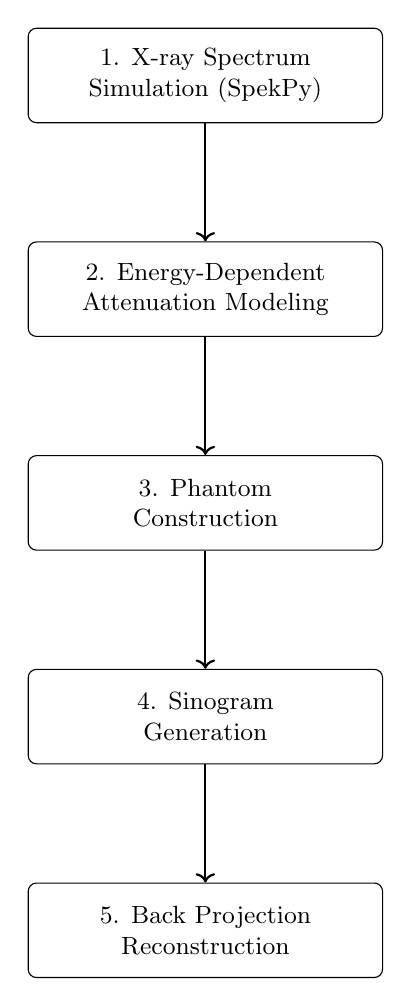
\begin{tikzpicture}[
    node distance=1.5cm and 2.2cm,
    box/.style={rectangle, draw, rounded corners=3pt, minimum width=4.5cm, minimum height=1.2cm, align=center, font=\small},
    arrow/.style={->, thick}
]

\node[box] (spectrum) {1. X-ray Spectrum \\ Simulation (SpekPy)};
\node[box, below=of spectrum] (attenuation) {2. Energy-Dependent \\ Attenuation Modeling};
\node[box, below=of attenuation] (phantom) {3. Phantom \\ Construction};
\node[box, below=of phantom] (sinogram) {4. Sinogram \\ Generation};
\node[box, below=of sinogram] (reconstruction) {5. Back Projection \\ Reconstruction};

\draw[arrow] (spectrum) -- (attenuation);
\draw[arrow] (attenuation) -- (phantom);
\draw[arrow] (phantom) -- (sinogram);
\draw[arrow] (sinogram) -- (reconstruction);

\end{tikzpicture}
\caption{Project Overview}
\label{fig:pipeline}
\end{figure}

\section{Methods}

\subsection{Background Physics}
\subsubsection{X-ray generation}
X-rays are produced in  a x-ray tube when high kinetic energy electrons are accelerated towards a positive anode. Tungsten is a common choice for the anode (due to its high melting point and high atomic number). Electrons come close to nuclei of the target, causing a deceleration and change in direction, converting kinetic energy into a spectrum of electromagnetic radiation. Incident electrons can ionise the material, removing an electron from the anode. As the electron orbit vacancy gets filled by a orbital shell electron in a further out shell a photon is emitted. As orbital energies and their differences are unique in atoms, this leads to what we call "characteristic radiation".
\cite{Tafti2023}

\begin{figure}
  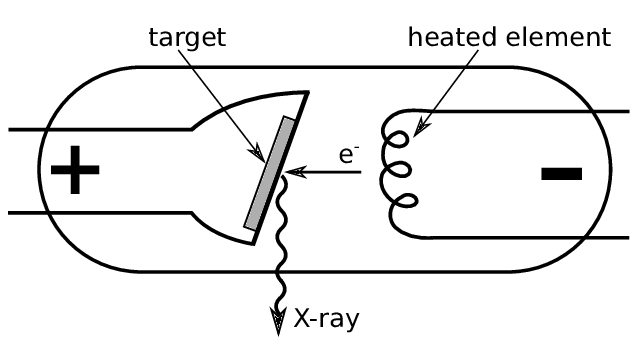
\includegraphics[width=\linewidth]{xray_tube.png}
  \caption{Schematic diagram of an X-ray tube, illustrating thermionic emission, electron acceleration, and the production of bremsstrahlung and characteristic radiation~\cite{Mason2018}.}
  \label{fig:X-ray tube}
\end{figure}

Figure \ref{fig:X-ray tube} shows a diagram of a x-ray tube where electrons are emitted via thermionic emission and then accelerated toward a positively charged anode, where their interactions with the target produce both bremsstrahlung and characteristic radiation.

An X-ray spectrum was simulated using \texttt{SpekPy}, a dedicated toolkit for modeling diagnostic X-ray tubes. 

For the simulation, a tungsten target and 150~kVp tube voltage were specified, and a 2.5~mm aluminium filter was applied to eliminate low-energy, non-diagnostic photons. These materials and values were chose to approximate conditions in general radiography. The filtered spectrum is shown in Figure~\ref{fig:basespectra}, where characteristic peaks corresponding to tungsten are clearly visible.

It is important however to critically consider these choices:

\begin{itemize}
	\item Tube voltage 150~kVp: This high voltage is commonly the upper limit for x-ray tubes in medical settings. Having such a high voltage increases the proportion of high energy photons and ensures that the characteristic peaks of tungsten (main peak at ~59 keV \cite{CharacteristicRadiation}). However in actual imaging to minimise radiation exposure, tube voltage varies depending on applications e.g. paediatric CT benefiting from lower potentials. 
	\item Aluminium filter 2.5mm: This simulates beam hardening by attenuating low-energy photons ($<30$ keV), which contribute little to image quality and increase patient dose. There is inherent filtration from the x-ray tube but added sheets are customised for individual examinations to take advantage of specific metals filtration characteristics to improve image quality. 2.5mm of aluminium is the minimum total filtration on x-ray tubes according to U.S. guidelines \cite{Filters}
\end{itemize}

Despite these simplifications, the generated spectrum demonstrates results that are suitable for the modelling carried out

\begin{figure}
	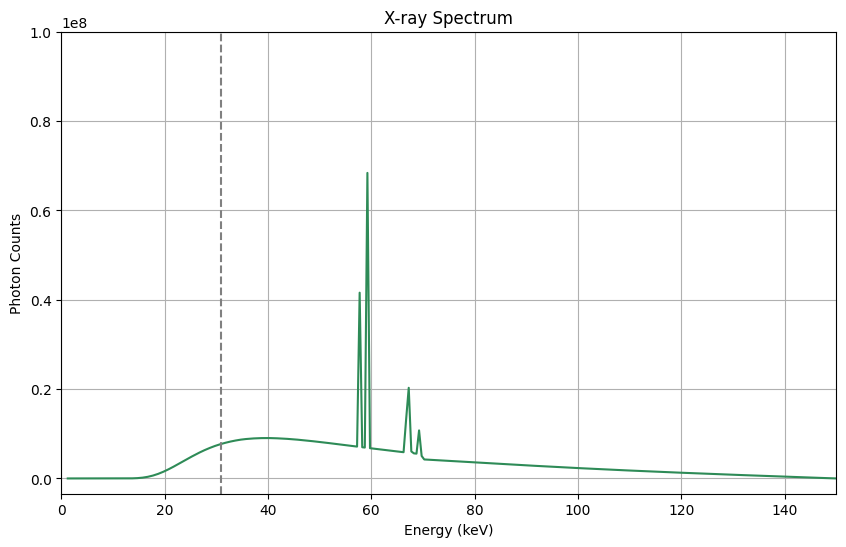
\includegraphics[scale=0.6]{typicalxrayspectra.png}
	\caption{Simulated X-ray spectrum from a tungsten target after 2~mm aluminium filtration. Characteristic peaks are visible at specific energy levels corresponding to tungsten.}
  \label{fig:basespectra}
\end{figure}

\subsubsection{Attenuation of X-rays}
As x-rays pass through matter, they are attenuated according to the Beer-Lambert law: 
\begin{equation} \label{bl}
I(E) = I_0 \cdot e^{-\mu(E) x}
\end{equation}

Where:
\begin{itemize}
  \item $I(E)$: Transmitted intensity at energy $E$
  \item $I_0(E)$: Incident intensity at energy $E$
  \item $\mu(E)$: Energy-dependent linear attenuation coefficient [cm$^{-1}$]
  \item $x$: Material thickness [cm]

\end{itemize}

The attenuation coefficient, $\mu$ is modelled as energy dependent to reflect real world phenomena such as beam hardening. The linear attenuation coefficient is computed from the mass attenuation coefficient, obtained from the NIST database~\cite{NISTXRay}, via:

\begin{equation} \label{linearatt}
\mu(E) = \left(\frac{\mu}{\rho}\right) \cdot \rho
\end{equation}
where $\left(\frac{\mu}{\rho}\right)(E)$ is the energy-dependent mass attenuation coefficient [cm$^2$/g], and $\rho$ is the physical density of the material [g/cm$^3$].

\subsection{Demonstrating Beam Hardening}
Beam hardening refers to the selective attenuation of low-energy photons leading to an effect similar to a high-pass filter in electronics. Beam hardening occurs during x-ray attenuation, as higher energy (hard) X-rays penetrate dense materials more effectively than the low energy (soft) X-rays. This has the effect of shifting the peak of the bremsstrahlung radiation towards higher energies. Since monochromatic beams do not exhibit this shift, characteristic peaks -arising from discrete atomic transitions— remain unaffected.

To model attenuation through  tissue, energy-dependent linear attenuation coefficients were computed from NIST mass attenuation data. After interpolating these coefficients to match the energy resolution of the spectrum, exponential attenuation was applied using the Beer-Lambert law in Equation~\ref{bl}.

Figure \ref{fig:beamhardening} shows beam hardening on the X-ray spectrum. The lower-energy (soft) x-rays are preferentially attenuated, resulting in a spectrum that is skewed toward higher energies. Lower-energy photons are absorbed more readily than high-energy ones. As a result, the transmitted spectrum becomes ”hardened” with its average energy increasing. We also don’t see any hardening for the monochromatic peaks, as monochromatic beams by definition do not change their average energy.

\begin{figure}[H]
	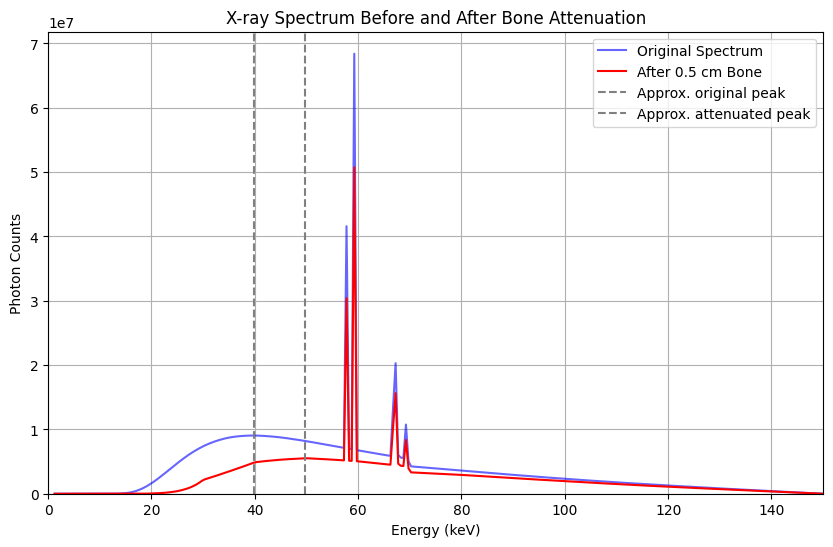
\includegraphics[scale=0.6]{beamhardening.png}
	\caption{Beam hardening visualized by comparing the X-ray spectrum before
and after passing through 0.5cm of bone. Low-energy components are preferen-
tially attenuated, resulting in a hardened spectrum.}
  \label{fig:beamhardening}
\end{figure}

Quantitatively:

\begin{table}[H]
\begin{tabular}{
>{\columncolor[HTML]{000000}}l ll}
\cellcolor[HTML]{FFFFFF}{\color[HTML]{FFFFFF} }      & \cellcolor[HTML]{000000}{\color[HTML]{FFFFFF} Before Attenuation} & \cellcolor[HTML]{000000}{\color[HTML]{FFFFFF} After Attenuation} \\
{\color[HTML]{FFFFFF} Peak energy (keV)}             & 39.8                                                              & 49.8                                                             \\
{\color[HTML]{FFFFFF} Mean energy (keV)}             & 60.27                                                             & 67.27                                                            \\
{\color[HTML]{FFFFFF} Spectral Hardness Ratio (SHR)} & 0.6110                                                            & 0.7434                                                          
\end{tabular}
\end{table}
The Spectral Hardness Ratio (SHR)-defined as the fraction of photons above 50 keV-increases from 0.6110 to 0.7434, quantitatively confirming that the spectrum becomes harder after transmission. These metrics demonstrate that beam hardening is a measurable shift in the spectrum

This hardening effect is critical in diagnostic imaging, as it alters tissue contrast and can introduce artefacts if not properly corrected in reconstruction algorithms. The most common CT beam hardening artefacts are:
\begin{itemize}
	\item Streaking artefacts, where dark bands appear between dense structures
	\item Cupping artefacts, where the center of a homogeneous object appears less attenuating than the edges
\end{itemize}
\cite{Murphy2016}.
\begin{figure}%
    \centering
    \subfloat[\centering CT streak artefact caused by gunshot bullets\cite{GunshotCase}.]{{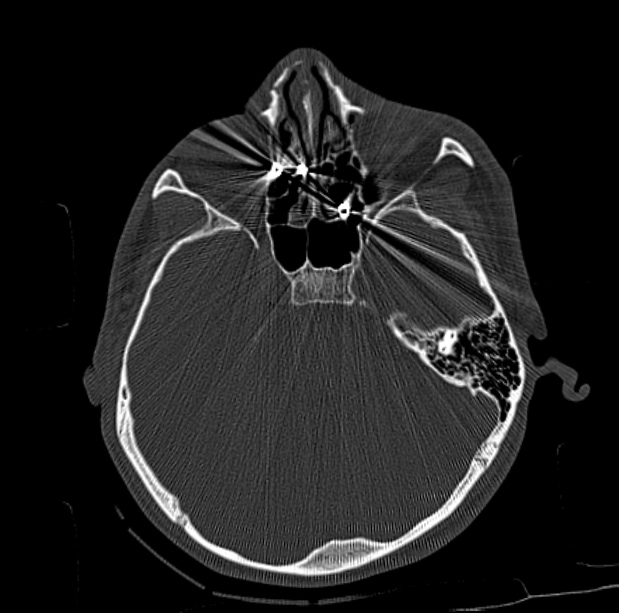
\includegraphics[width=5cm]{streakingartefact.jpg} }}%
    \qquad
    \subfloat[\centering CT cupping artefact, grey matter appears artifactually and symmetrically hypodense\cite{CuppingArtifact}.]{{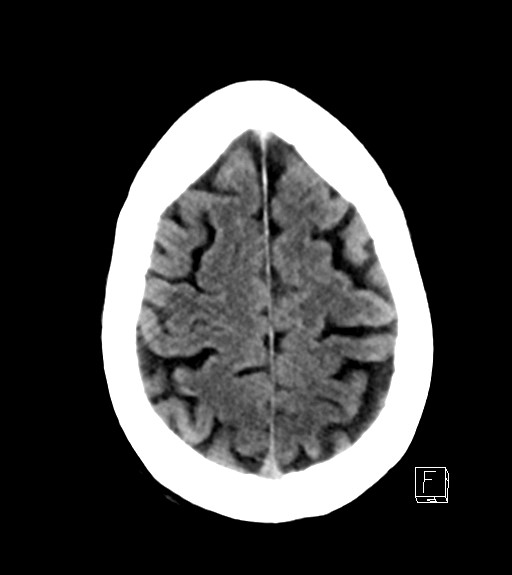
\includegraphics[width=5cm]{cuppingartefact.jpg} }}%
    \caption{2 Figures side by side}%
    \label{fig:example}%
\end{figure}

\subsection{Phantoms and Sinograms}
\subsubsection{Generating Phantoms}
In medical imaging, phantoms are used as stand-ins for human tissues to test and validate imaging systems and reconstruction algorithms. They allow for controlled experimentation as the 'ground truth' is always known. A widely used model is the Shepp-Logan phantom \cite{Shepp1974}, serving as a model of the human head and defined as 10 ellipses with varying parameters and intensity.

To generate this model, a Python implementation by Jan Hrach~\cite{HrachovecPhantom} was adapted. The phantom is represented as a 2D array with constant attenuation coefficients across the image, making it ideal for examining reconstruction quality under monoenergetic or simplified polychromatic assumptions.

To complement this, a second phantom was constructed with a simplified geometry: a circular region representing soft tissue (low attenuation). Unlike the Shepp–Logan model, this phantom is explicitly designed for use with energy-dependent attenuation data with goals of showing beam hardening artefacts.

Circular regions were defined using a Boolean masking function and the phantom was initialized as a 3D array to accommodate energy-resolved attenuation data:

\begin{figure}[H]
	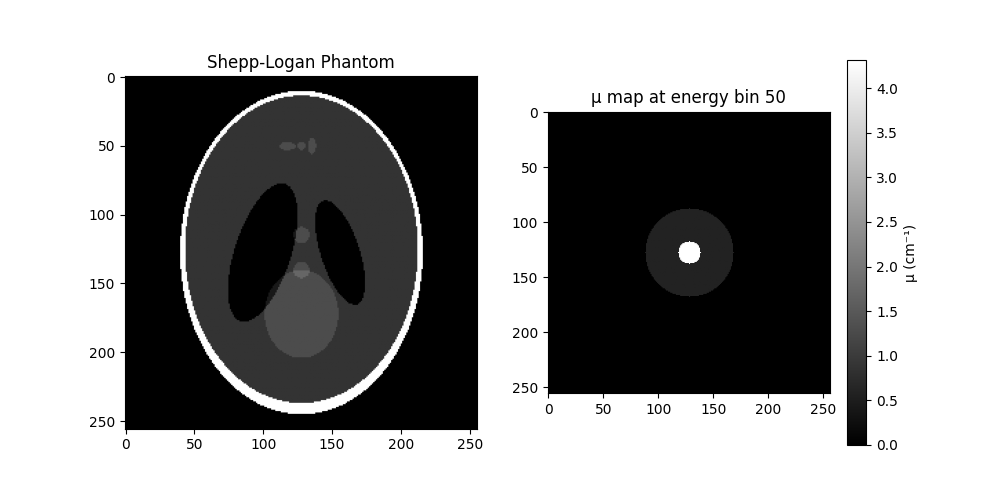
\includegraphics[width=\linewidth]{simplephantom.png}
	\caption{Left: Shepp-Logan phantom. Right: Circular phantom with energy dependent attenuation($\mu$ map at energy bin 50).}
	\label{fig:phantoms}
\end{figure}

\subsubsection{Sinograms}
\label{sinogramsec}
A sinogram is a 2D representation of the projection data acquired in a CT scan, where each row corresponds to a 1D projection taken at a specific angle. Before we can reconstruct the cross-sectional image of the scanned object, the initial x-ray attenuation measurements are compiled into this sinogram format.

To understand image reconstruction, we need to define projections. A projection in CT scans represents the total attenuation of x-rays along a specific path of the object, mathematically this is represented as a line integral. At an angle $\theta$, the parallel beam geometry represents a new coordinate system $(r, s)$ in which the intensity profile $I_\theta (r)$ is measured. Other beam geometries such as fan or cone geometries require different methodology.

$$\begin{pmatrix} r \\ s \end{pmatrix} = R \begin{pmatrix} x \\ y \end{pmatrix} = \begin{pmatrix} \cos\theta & \sin\theta \\ -\sin\theta & \cos\theta \end{pmatrix} \begin{pmatrix} x \\ y \end{pmatrix}$$

Conversely,
$$\begin{pmatrix} x \\ y \end{pmatrix} = R^T \begin{pmatrix} r \\ s \end{pmatrix} = \begin{pmatrix} \cos\theta & -\sin\theta \\ \sin\theta & \cos\theta \end{pmatrix} \begin{pmatrix} r \\ s \end{pmatrix}$$

\begin{figure}[H]
	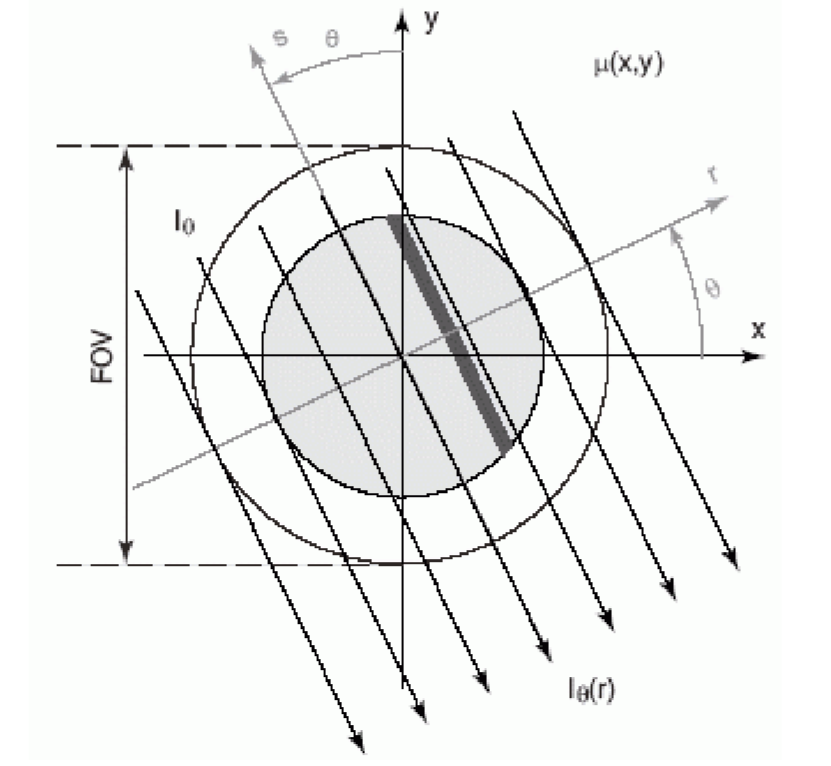
\includegraphics[scale=0.6]{coordinate_system.png}
	\caption{The object is defined in the Cartesian coordinate system $(x,y)$. For a projection at angle $\theta$, a new coordinate system $(r,s)$ is defined, where r is the perpendicular distance from the origin to the x-ray ray, and s is the coordinate along the ray path}
	\label{fig:coord}
\end{figure}

With parallel beams at a fixed angle $\theta$, the measured intensity at position $r$ along $L_{(r,\theta)}$ is given by the Beer-Lambert law:

\begin{align}
I_{\theta}(r) &= I_0 \cdot \exp\Bigl({-\int\limits_{L_{(r,\theta)}} \mu (x,y) ds} \Bigr) \\
& = I_0 \cdot \exp\Bigl({-\int\limits_{L_{(r,\theta)}} \mu \left(r \cos(\theta) - s \sin(\theta),r \sin(\theta) + s \cos(\theta)\right) ds} \Bigr) 
\end{align}

Each Intensity profile $I_\theta (r)$ is transformed into an attenuation profile $p_\theta (r)$, by taking the negative natural logarithm of the ratio of transmitted intensity to incident intensity:

\begin{align}
p_\theta (r) = - \ln \frac{I_\theta (r)}{I_0} = -\int\limits_{L_{(r,\theta)}} \mu \left(r \cos(\theta) - s \sin(\theta),r \sin(\theta) + s \cos(\theta)\right) ds
\end{align}

This attenuation profile is what our detector measures at each angle.

Plotting our result we get:
\begin{figure}[H]
	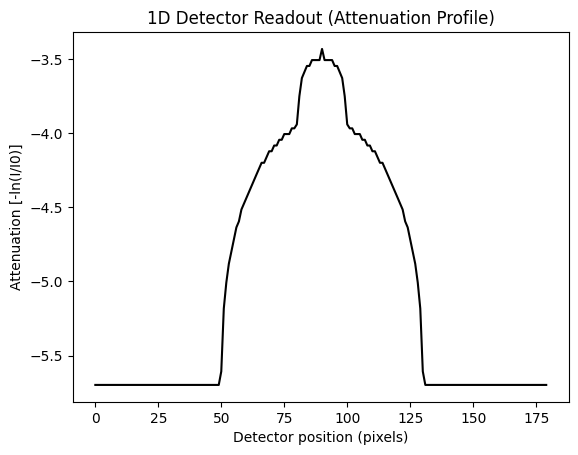
\includegraphics[scale=0.6]{detectorreadout.png}
	\caption{1D detector readout for our circular phantom.}
	\label{fig:detector1d}
\end{figure}

If we arrange projections from all angles (only $(0,\pi)$ as $(\pi, 2\pi)$ are redundant for parallel beams) side by side as a 2D image, we get a sinogram. We can view this 2D dataset $p(r, \theta)$ for our circular phantom in Figure \ref{fig:sinogramcircle}, this sinogram was generated using scipy.ndimage.rotate to simulate the projections. While convenient, using scipy.ndimage.rotate is not the ideal choice as it introduces interpolation artefacts. This means that the "ray paths" are not perfectly straight lines of integration but rather interpolated paths, which can introduce smoothing or blurring. A more accurate sinogram model would use a more direct ray-tracing algorithm, such as Siddons' \cite{Siddon1985}. However, for this fundamental demonstration, the conceptual understanding provided by this approach is sufficient.

Another, more interesting sinogram can be found from our more complex Shepp-Logan phantom, which we can see in Figure \ref{fig:sinogramshepp}. We can notice sinusoidal curves throughout the image, motivating the name sinogram. Each point or localized structure in the (x,y) domain traces a sinusoidal path in the sinogram because the distance $r$ from the origin to the projection line changes with angle according to a sine-cosine relationship. Specifically, a fixed point $(x_0, y_0)$ in the object maps to a curve defined by $r = x_0 \cos \theta + y_0 \sin \theta$, which is inherently sinusoidal in $\theta$.

\begin{figure}[H]
	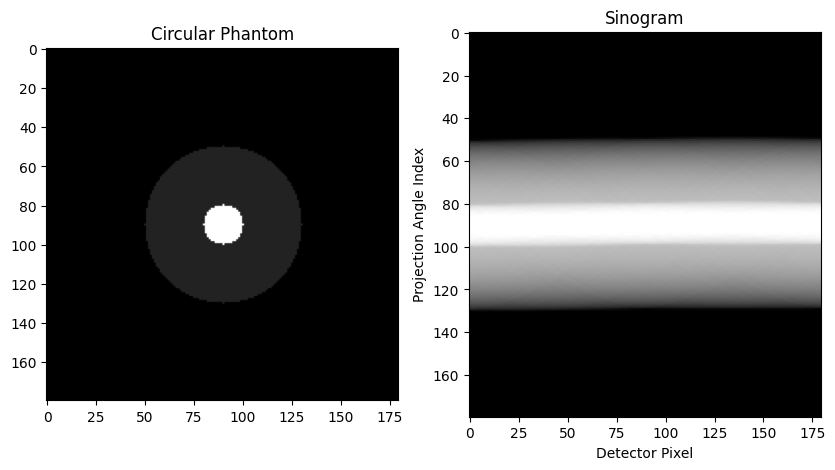
\includegraphics[scale=0.5]{sinogramcircle.png}
	\caption{Sinogram for our circular phantom, note how it is constant in $\theta$ due to the rotational symmetry of the circle.}
	\label{fig:sinogramcircle}
\end{figure}

\begin{figure}[H]
	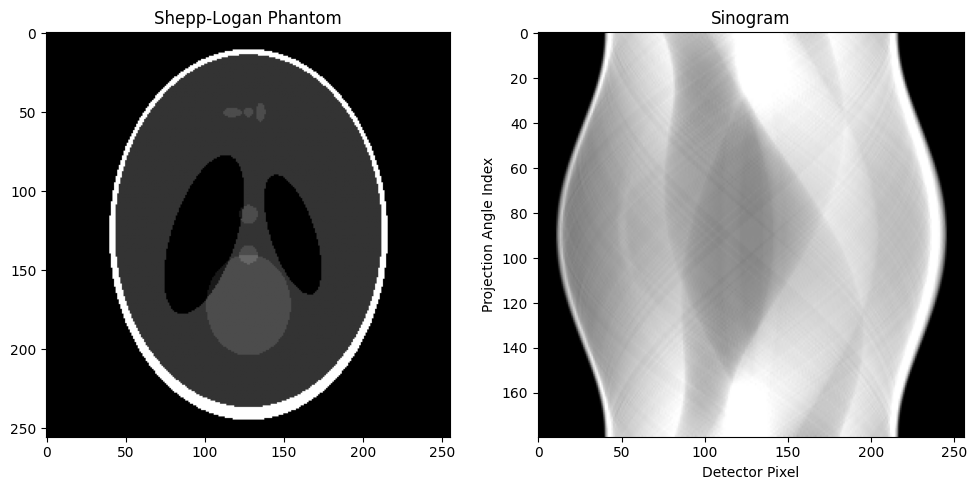
\includegraphics[scale=0.5]{sinogramshepp.png}
	\caption{Sinogram for the Shepp-Logan phantom.}
	\label{fig:sinogramshepp}
\end{figure}

The transformation of a function $\mu (x,y)$ into $p(r, \theta)$, is known as the Radon transform defined here as:
\begin{definition}
For a function $\mu(x,y)$ defined on $\mathbb{R}^2$, the Radon transform of $\mu$, denoted as $\mathcal{R}\left\{\mu \right\}$, is defined as
\begin{align*}
p(r, \theta) &= \mathcal{R} \left\{ \mu(x,y) \right\} \notag \\
             &= \int_{-\infty}^{\infty} \mu(r \cos\theta - s \sin\theta,\; r \sin\theta + s \cos\theta) \, ds
\end{align*}
\label{radon}
\end{definition}
We can therefore phrase the problem of CT reconstruction as finding an inversion formula for the Radon transform \cite{Beatty2012}. 

\subsection{Inverse Radon Transform and Back Projection}
\subsubsection{Simple Back Projection}
One intuitive way we can think of image reconstruction is with 'Simple Back Projection'. If we take each projection $p_\theta (r)$ of our sinogram, and smear the value along lines perpendicular to the angle $\theta$ and add these up for all $\theta$ before normalising we should get back to our result. Imagine each projection as a shadow cast from a specific direction; by stacking up these shadows, we can approximate the object that cast them.
Mathematically, we define the back projection as:
\begin{definition}
Let $p = p(r, \theta)$. We define the back projection, $\mathcal{B} p$, at a point $(x,y)$ as
$$
\mathcal{B} p(x,y) = \frac{1}{\pi} \int_{0}^{\pi} p(x \cos(\theta) + y \sin(\theta), \theta) d\theta
$$
\label{backprojection}
\end{definition}

In practice, we implement this by:
\begin{itemize}
	\item Taking each row of the sinogram (a projection)
	\item Replicating it across a 2D grid (smearing)
	\item Rotating it back in place
	\item Summing the results across all angles
\end{itemize}

\begin{figure}[H]
	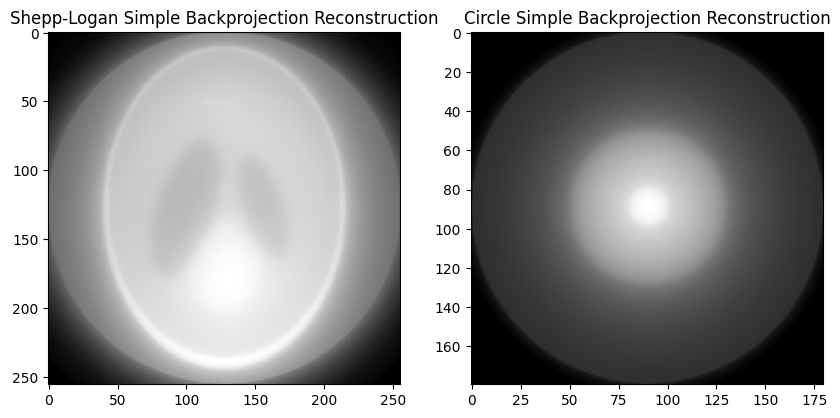
\includegraphics[width=\linewidth]{sbpreconstructions.png}
	\caption{Simple Back Projection Reconstructions for our 2 phantoms.}
	\label{fig:SBPreconstructions}
\end{figure}

This roughly reconstructs the structure of the phantoms and we can make out some of the internal structure in both of our phantoms. Both of our phantoms are blurred and have pronounced dark corners. 

The dark corners can be explained quantitatively, as they receive fewer ray contributions when we rotate around but to understand the blurring we need to requires further mathematical understanding. In our circle phantom, we can see a cupping artefact as the centre is brighter than it should be, due to ray-hardening.

Doing more quantitative analysis on how our Shepp-Logan reconstruction compares to the original we can compare Mean Square Error (MSE) and Structural Similarity Index Measure (SSIM) \cite{Sara2019}, for our Shepp-Logan:
\begin{itemize}
	\item MSE: 0.3778
	\item SSIM: 0.3130
\end{itemize}

In order to get these figures I ensured that both the original image and reconstruction was normalised, and applied a circle masking function to ensure we were only comparing the significant parts of the image and not the darkened corners.

MSE measures the average squared difference between actual and ideal pixel values. Since the normalized image ranges from 0 to 1, an MSE of 0.3778 is very high, indicating a substantial loss of pixel-wise fidelity.

SSIM evaluates image quality by considering luminance, contrast and structural information. A value close to 1 would imply the 2 images are similar, so 0.3130 suggests significant degradation in these areas (which matches what we observe). The threshhold is usually $> 0.9$ for high quality reconstructions.

Overall quantitative image comparison is a tricky topic and both of these metrics have issues \cite{Nilsson2020}, but they still clearly indicate the need for a more sophisticated reconstruction algorithm. As we can see, simple back projection cannot be the inverse transformation we are looking for, the observed blurring are not just empirical observations but direct consequences of the mathematical operation underlying SBP.

\subsection{Fourier Slice Theorem and Filtered Back Projection}
\subsubsection{The Fourier Slice Theorem}
To rigorously understand why simple back projection leads to blurring, we first prove the Fourier slice theorem, which gives a relationship between the one dimensional Fourier transform of the Radon transform and the two dimensional Fourier transform.

Recall,
\begin{definition}
For a given absolutely integrable function $f$ on $\mathbb{R}$ the Fourier transform of $f$ given by $\mathcal{F}f$ is defined for every real number $\omega$ as:
$$
\mathcal{F}f(\omega) = \int_{-\infty}^{\infty} f(x) e^{- i \omega x}dx
$$
\end{definition}

We also define the inverse Fourier transform as:

\begin{definition}
For a given absolutely integrable function $f$ on $\mathbb{R}$ we define the inverse Fourier transform of $f$ given by $\mathcal{F}^{-1}f$ evaluated at $x$ as:
$$
\mathcal{F}^{-1}f(x) = \frac{1}{2 \pi} \int_{-\infty}^{\infty} f(\omega) e^{i \omega x}d\omega
$$
\end{definition}

Analogously in 2 dimensions:
\begin{definition}
For a given absolutely integrable function $g$ on $\mathbb{R} ^ 2$ the 2 dimensional Fourier transform of $g$ given by $\mathcal{F}_2 g$ is defined all $X, Y \in \mathbb{R} ^ 2$ as:
$$
\mathcal{F}_2 g(X, Y) =  \int_{-\infty}^{\infty} \int_{-\infty}^{\infty} g(x, y) e^{- i (x X + yY)}dxdy
$$
\label{2dfourier}
\end{definition}

We similarly define the inverse Fourier transform on $\mathbb{R}^2$.

\begin{definition}
For a given absolutely integrable function $g$ on $\mathbb{R} ^ 2$ the 2 dimensional inverse Fourier transform at a point $(x,y)$ denoted by $\mathcal{F}_2 ^{-1} g(x,y)$ is given as:
$$
\mathcal{F}_2 ^{-1} g(x, y) = \frac{1}{4 \pi^2} \int_{-\infty}^{\infty} \int_{-\infty}^{\infty} g(X, Y) e^{i (x X + yY)}dxdy
$$
\end{definition}

We can now state the Fourier slice theorem.
\begin{theorem}
For an absolutely integrable function $f$ defined on $\mathbb{R}^2$ and all $S \in \mathbb{R}$ and all $\theta \in \left[ 0, 2\pi \right)$,
$$
\mathcal{F}_2 f(S \cos \theta, S \sin \theta) = \mathcal{F}(\mathcal{R}f)(S, \theta)
$$
\label{cslice}
\end{theorem}
\begin{proof} 
First, by definition \ref{2dfourier}:
$$
\mathcal{F}_2 f(S \cos \theta, S \sin \theta) =  \int_{-\infty}^{\infty} \int_{-\infty}^{\infty} f(x, y) e^{- i S(x \cos \theta + y \sin \theta )}dxdy
$$ \label{fslice}
We can know  implement the change of variables defined in Section \ref{sinogramsec} \\
$x(s) = r \cos \theta - s \sin \theta$ and $y(s) = r \sin \theta + s \cos \theta$, where $r = x \cos \theta + y \sin \theta$
Looking at the determinant for the Jacobian of $x(s)$ and $y(s)$:
$$
\det \begin{pmatrix}
       \frac{\partial x}{\partial r} & \frac{\partial x}{\partial s} \\
       \frac{\partial y}{\partial r} & \frac{\partial y}{\partial s}
   \end{pmatrix} = 1
$$
So we can say, $dsdr = dxdy$. We therefore write the right side of equation \ref{fslice} as:
$$
\int_{-\infty}^{\infty} \int_{-\infty}^{\infty} f(r \cos \theta - s \sin \theta, r \sin \theta + s \cos \theta) e^{- i S r}dsdr
$$
Which we can rearrange as:
$$
\int_{-\infty}^{\infty} \left( \int_{-\infty}^{\infty} f(r \cos \theta - s \sin \theta, r \sin \theta + s \cos \theta)ds  \right) e^{- i S r}dr
\label{innerintegral}
$$
The inner integral is the Radon transform of $f$ as defined by Definition \ref{radon}. Therefore equation \ref{innerintegral} can be written as:
$$
\int_{-\infty}^{\infty} \left( \mathcal{R} f (r, \theta) \right) e^{- i S r}dr
$$
Which is just the definition of the Fourier transform of $\mathcal{R} f$ evaluated at $(S, \theta)$\\
Therefore:
$$
\mathcal{F}_2 f(S \cos \theta, S \sin \theta) = \mathcal{F}(\mathcal{R}f)(S, \theta)
$$
\end{proof}

\begin{figure}[H]
	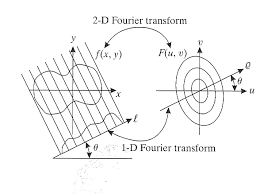
\includegraphics[width=\linewidth]{fourierslicetheorem.jpg}
	\caption{Fourier slice theorem visualisation. We can see the relationship between the projections 1D Fourier transform and the functions 2D Fourier transform. }
	\label{fourierslicetheorem}
\end{figure}

This relationship is incredibly useful in medical imaging, in words: the one dimensional Fourier transform of the projection of a function (recall this is what the Radon transform is) is equal to a slice through the origin, parallel to the line we projected our function on of the 2D Fourier transform of the function. This relationship is visualised in figure \ref{fourierslicetheorem}.

\subsubsection{The Filtered Back Projection Formula}
We can use this to define the filtered back projection formula.
\begin{theorem}
For an absolutely integrable function $f$ defined on $\mathbb{R}^2$
$$
f(x,y) = \frac{1}{2} \mathcal{B} \left\lbrace \mathcal{F}^{-1} \left[ |S| \mathcal{F} \left( \mathcal{R}f \right) \left( S, \theta \right) \right] \right\rbrace (x,y)
$$
\end{theorem}
\begin{proof}
For the 2 dimensional Fourier transform and its inverse:
\begin{align}
f(x,y) &= \mathcal{F}_2^{-1} \mathcal{F}_2 f(x,y) \\
&= \frac{1}{4 \pi^2} \int_{-\infty}^{\infty} \int_{-\infty}^{\infty} \mathcal{F}_2 f(X, Y) e^{i (x X + yY)}dXdY
\end{align}
We can then use a change of variables from Cartesian to polar coordinates.
$X = S \cos \theta$, $Y = S \sin \theta$, with Jacobian determinant $dXdY = |S| dS  d\theta$ to get:
$$
f(x,y) = \frac{1}{4 \pi^2} \int_{0}^{\pi} \int_{-\infty}^{\infty} \mathcal{F}_2 f(S \cos \theta, S \sin \theta) e^{i S(x \cos \theta + y \sin \theta)} |S|dSd\theta
$$
Using the Central Slice Theorem \ref{cslice} we see:
$$
f(x,y) = \frac{1}{4 \pi^2} \int_{0}^{\pi} \int_{-\infty}^{\infty} \mathcal{F}(\mathcal{R} f(S , \theta)) e^{i S(x \cos \theta + y \sin \theta)} |S|dSd\theta
$$
Analysing the inner integral:
\begin{align*}
\int_{-\infty}^{\infty} \mathcal{F}(\mathcal{R} f(S , \theta)) e^{i S(x \cos \theta + y \sin \theta)} |S|dS \\
= 2\pi \left( \frac{1}{2 \pi} \int_{-\infty}^{\infty} \mathcal{F}(\mathcal{R} f(S , \theta)) e^{i S(x \cos \theta + y \sin \theta)} |S|dS \right) \\
= 2\pi \mathcal{F}^{-1} \left[ |S| \mathcal{F} \left( \mathcal{R}f \right) \left( S, \theta \right) \right] (x \cos \theta + y \sin \theta, \theta)
\end{align*}

Which allows us to write:
$$
f(x,y) = \frac{1}{2 \pi} \int_{0}^{\pi} \mathcal{F}^{-1} \left[ |S| \mathcal{F} \left( \mathcal{R}f \right) \left( S, \theta \right) \right] (x \cos \theta + y \sin \theta, \theta) d\theta
$$
Which using our Backprojection formula from Definition \ref{backprojection} we can simplify to:

$$
f(x,y) = \frac{1}{2} \mathcal{B} \left\lbrace \mathcal{F}^{-1} \left[ |S| \mathcal{F} \left( \mathcal{R}f \right) \left( S, \theta \right) \right] \right\rbrace (x,y)
$$
\end{proof}

We call the $|S|$ multiplier in this formula a filter. We can actually get this formula in a simpler form by supposing there exists some function $\phi(t)$ such that $\mathcal{F}\phi (S) = |S|$ and say:
$$
f(x,y) = \frac{1}{2} \mathcal{B} \left\lbrace \mathcal{F}^{-1} \left[ \mathcal{F}\phi \cdot \mathcal{F} \left( \mathcal{R}f \right) \left( S, \theta \right) \right] \right\rbrace (x,y)
$$
Using the Convolution Theorem \cite{wolfram_convolution} we therefore have:
\begin{align*}
f(x,y) &= \frac{1}{2} \mathcal{B} \left\lbrace \mathcal{F}^{-1} \left[ \mathcal{F} \left(\phi \star \mathcal{R}f \right) \left( S, \theta \right) \right] \right\rbrace (x,y) \\
&= \frac{1}{2} \mathcal{B} \left(\phi \star \mathcal{R}f \right) (x,y)
\end{align*}

This is great! We just need to filter our measured data $\mathcal{R}f$ with our function $\phi$ and then apply the back projection formula. However, there are no functions $\phi$ that satisfies $\mathcal{F} \phi(S) = |S|$, Consider:
$$
\mathcal{F}\phi(S) = \int_{-\infty}^{\infty} \phi(x)e^{-iSx} dx
$$
in the limit $S \to \infty$, $\mathcal{F}\phi \to 0$, but for the absolute value function $|S| \to \infty$. Meaning we cannot find a suitable function $\phi$ that satisfies for all $S$, 
$$\mathcal{F}\phi(S) = |S|$$.

\subsubsection{Practical Filtering}

\bibliography{References}
\bibliographystyle{ieeetr}
\end{document}
